%%
%% This is file `sample-sigconf.tex',
%% generated with the docstrip utility.
%%
%% The original source files were:
%%
%% samples.dtx  (with options: `sigconf')
%%
%% IMPORTANT NOTICE:
%%
%% For the copyright see the source file.
%%
%% Any modified versions of this file must be renamed
%% with new filenames distinct from sample-sigconf.tex.
%%
%% For distribution of the original source see the terms
%% for copying and modification in the file samples.dtx.
%%
%% This generated file may be distributed as long as the
%% original source files, as listed above, are part of the
%% same distribution. (The sources need not necessarily be
%% in the same archive or directory.)
%%
%% The first command in your LaTeX source must be the \documentclass command.
\documentclass[sigconf,nonacm]{acmart}

\usepackage[utf8]{inputenc}
\usepackage{multirow}
\usepackage[inline]{enumitem}

\settopmatter{printacmref=false} % Removes citation information below abstract
\renewcommand\footnotetextcopyrightpermission[1]{} % removes footnote with conference information in first column

\newcommand\note[2]{{\color{#1}#2}}
\newcommand\todo[1]{{\note{red}{TODO: #1}}}

%%
%% \BibTeX command to typeset BibTeX logo in the docs
\AtBeginDocument{%
  \providecommand\BibTeX{{%
    \normalfont B\kern-0.5em{\scshape i\kern-0.25em b}\kern-0.8em\TeX}}}


%%
%% Submission ID.
%% Use this when submitting an article to a sponsored event. You'll
%% receive a unique submission ID from the organizers
%% of the event, and this ID should be used as the parameter to this command.
%%\acmSubmissionID{123-A56-BU3}

%%
%% The majority of ACM publications use numbered citations and
%% references.  The command \citestyle{authoryear} switches to the
%% "author year" style.
%%
%% If you are preparing content for an event
%% sponsored by ACM SIGGRAPH, you must use the "author year" style of
%% citations and references.
%% Uncommenting
%% the next command will enable that style.
%%\citestyle{acmauthoryear}

%%
%% end of the preamble, start of the body of the document source.
\begin{document}

%%
%% The "title" command has an optional parameter,
%% allowing the author to define a "short title" to be used in page headers.
\title{Assignment 3}

%%
%% The "author" command and its associated commands are used to define
%% the authors and their affiliations.
%% Of note is the shared affiliation of the first two authors, and the
%% "authornote" and "authornotemark" commands
%% used to denote shared contribution to the research.
\author{Alexander Hartl (e01125115)}
\authornote{Both authors contributed equally to this research.}
%\email{alexander.hartl@tuwien.ac.at}

\author{Maximilian Bachl (e01100143)}
%\authornote[1]{Both authors contributed equally to this research.}
\authornotemark[1]
%\email{maximilian.bachl@gmail.com}

%%
%% By default, the full list of authors will be used in the page
%% headers. Often, this list is too long, and will overlap
%% other information printed in the page headers. This command allows
%% the author to define a more concise list
%% of authors' names for this purpose.
\renewcommand{\shortauthors}{Hartl and Bachl}

%%
%% The abstract is a short summary of the work to be presented in the
%% article.
%\begin{abstract}
%  A clear and well-documented \LaTeX\ document is presented as an
%  article formatted for publication by ACM in a conference proceedings
%  or journal publication. Based on the ``acmart'' document class, this
%  article presents and explains many of the common variations, as well
%  as many of the formatting elements an author may use in the
%  preparation of the documentation of their work.
%\end{abstract}

\settopmatter{printfolios=true}
\maketitle

\todo{Legend in some figures is misplaced}

\section{Introduction}

There is a significant body of scientific work focusing on the detection of unwanted behavior in networks. In the past, a viable way of performing intrusion detection was to inspect the content of packets themselves and detect if a packet delivers potentially harmful content.

More recently, with the rise of omnipresent encryption, available features have changed. Since payload is not available anymore, the focus now lies on features that are always available to observers such as port numbers, flags of packets etc. Network communication is usually grouped into \textit{flows}, which is commonly defined as a sequence of packets between two applications that may be located at different physical locations.

When analyzing flows, not only the aforementioned features are available but also features related to the timing of the individual packets as well as their size. For example, a specific attack might require the attacker to send three small packets and the victim to reply with two large packets followed by a small one the attacker. Various approaches have been proposed to extract features from flows and then perform anomaly detection with the results \cite{meghdouri_analysis_2018}. While this approach works well, it is problematic that first the whole flow has to be received and only afterwards it can be determined if there was an anomaly.

Thus, we design a network anomaly detection system that operates on a per-packet basis and decides if a packet is anomalous based on features that are available for traffic that is encrypted above the transport layer, like for example TLS or QUIC.
%rax
We show that our system has similar performance to other flow-based anomaly detection systems but can commonly detect anomalies before the flow is over. Using several explainability methods we show the different characteristics of different attacks and how many packets it takes on average to detect them.

Last, we explore the question whether adversarial samples can be found for this type of data. This is not a trivially answerable question since adversarial samples have mostly been analyzed in the context of computer vision. Our scenario significantly deviates from this in several ways because \begin{enumerate*}
\item the number of features is significantly smaller and
\item only certain features can be manipulated (for example the destination port cannot be manipulated)
\end{enumerate*}.

\section{RNN-based classifier}

\begin{table}[b]
\caption{Occurence probability of attack types.} \label{tab:occurrence}
\begin{tabular}{l r} \toprule
Attack type & Proportion \\
\midrule
Normal                                                         & $0.747468$ \\
DoS / DDoS:DoS Hulk                                            & $0.101014$ \\
PortScan:PortScan - Firewall off                               & $0.069020$ \\
DDoS:LOIT                                                      & $0.040784$ \\
Infiltration:Dropbox download & $0.032982$ \\
DoS / DDoS:DoS GoldenEye                                       & $0.003224$ \\
DoS / DDoS:DoS Slowhttptest                                    & $0.001819$ \\
DoS / DDoS:DoS slowloris                                       & $0.001680$ \\
Brute Force:SSH-Patator                                        & $0.001107$ \\
Botnet:ARES                                                    & $0.000327$ \\
Web Attack:XSS                                                 & $0.000293$ \\
PortScan:PortScan - Firewall on                                & $0.000165$ \\
Brute Force:FTP-Patator                                        & $0.000110$ \\
Web Attack:Sql Injection                                       & $0.000006$ \\
DoS / DDoS:Heartbleed                                          & $0.000001$ \\
\bottomrule
\end{tabular}
\label{tab:occurence}
\end{table}

The dataset we use is the \textit{CIC-IDS 2017} dataset \cite{sharafaldin_toward_2018}, which includes the attacks listed in \autoref{tab:occurence} and contains over two million flows in total. We implement an LSTM-based classifier with three layers of 512 neurons each. As the input features we use \begin{itemize*}
\item source port
\item destination port
\item protocol identifier
\item packet sizes
\item interarrival times of packets
\item packet directions (if packet goes there or back)
\item all TCP flags (0 if flow is not TCP)
\end{itemize*}. Of these features, source port, destination port and protocol identifier are constant over the whole flow while the others vary.

We use Z-score normalization and a train/test split of 2:1.

\autoref{tab:performance_results} shows that our classifier achieves an accuracy that is similar to the one of the random forest and the multilayer perceptron that we developed in the previous exercise. However unlike these classifiers, our recurrent classifier has the advantage that it can detect attacks already before they are over.

\begin{table}
\caption{Detection performance results. Random forest and Multilayer Perceptron are from the previous exercise, LSTM is this implementation.} \label{tab:performance_results}
\begin{tabular}{l r r r} \toprule
& RF & MLP & LSTM \\ \midrule
Accuracy	&	0.9974 & 0.9970	& 0.9947 \\
Precision	&	0.9965 & 0.9979 & 0.9894	\\
Recall	&	0.9931 & 0.9903	& 0.9897 \\
F1	&	0.9948 & 0.9941	& 0.9896 \\
Youden	&	0.9920 & 0.9896 & 0.9861 \\
\bottomrule
\end{tabular}
\end{table}

\section{Explaining Recurrent Neural Networks}
From a naive perspective, one might be tempted to reuse explainability methods for recurrent neural networks by considering a flow the sum of its packet features.
We identify several problems which occur when trying to explain decisions made by recurrent neural networks.

\begin{itemize}
\item
\textbf{Feature quantity.}
The number of features that is fed into a recurrent neural network is found as the product of packet features with the total length of the flow. For long flows, the total number of inputs can therefore grow to a substantial size.

\item
\textbf{Variable sequence lengths.}
The length of different flows might differ tremendously. Hence, features which are important for the network's outcome for one sequence might not even exist for other flows. Furthermore, the question arises how the distance between flows of different length can be computed.

\item
\textbf{Lack of a distance measure.}
However, even if we restricted our analysis to flows of a constant length, a flow is different from the plain concatenation of its packet features.
If we, for example, consider a classification problem as in this document, we expect that after a certain amount of time steps the classifier is able to perform the classification with a certain confidence. Arguably, features at the beginning of a flow are thus more important for the classifier. Giving differences at the end of a sequence the same weight as differences at its beginning, therefore seems incorrect.

\item
\textbf{Multiple prediction outputs.}
Often a recurrent neural network produces an output at each time step. When trying to apply explainability methods, hence, the question arises which prediction to base the methods on.

The natural choice is to base the methods on the prediction output which occurs at the same time step as the feature under investigation. Not only does this approach require a substantially lower amount of computational ressources compared to predictions occuring at a later time step, but we also expect the immediately occuring prediction outome to exhibit a stronger correlation to the feature under investigation than a prediction outcome which occuring many time steps later. However, due to the complex decision processes that can occur for deep neural networks, it is absolutely  uncertain if the network's final prediction is correctly depicted when following this approach.
\end{itemize}

\subsection{Feature Importance Metrics}
\begin{table}
\caption{Accuracy drop when replacing feature values with random data.}
\label{tab:feat_importance}
\begin{tabular}{l r}
\toprule
Feature & Accuracy drop \\ \midrule
Protocol	&	0.1323	\\
Packet Length	&	0.1203	\\
SYN Flag	&	0.1067	\\
ACK Flag	&	0.0805	\\
Destination port	&	0.0796	\\
PSH Flag	&	0.0767	\\
Direction	&	0.0732	\\
Source port	&	0.0254	\\
Interarrival time	&	0.0200	\\
RST Flag	&	0.0116	\\
FIN Flag	&	0.0100	\\
ECE	Flag &	0.0000	\\
URG Flag	&	0.0000	\\
CWR Flag	&	0.0000	\\
NS Flag	&	0.0000	\\
\bottomrule
\end{tabular}
\end{table}
As a first step to understanding the neural network's decisions, we tried to estimate how important individual features are for the model's predictions.

To this end, we evaluated by what extent detection accuracy drops when withholding individual features from the classifier. We thus replaced values of individual features by values randomly drawn from the same distribution as the real feature values. We ensured that features which stay constant for a flow, i.e. source port, destination port and protocol, also stay constant for the distorted flows.

\autoref{tab:feat_importance} shows our results. The results match to a large extent with the expectations one has when classifying network flows. In particular,  the most important features turn out to be the used protocol, packet length and the SYN TCP flag. While the first two features are essential for characterizing flows, a high number of packets with set SYN flag is an important characteristic for port scanning or certain DoS attacks.

Also the fact that most of TCP flags do not play an important role in our dataset, was expected.
It is interesting to note, however, that the interarrival time of packets does not play a crucial role for the detection of attacks.

\subsection{Explainability Plots}
During flow extraction we used a usual 5-tuple flow key, which distinguishes flows based on the protocol they use and their source and destination port and IP address. Hence, these features are constant for all packets in one flow, which allows us to use explainability methods which have been proposed for non-recurrent classification methods.

In particular,  in literature the use of Partial Dependency Plots (PDP) is proposed. If $\boldsymbol X \in \mathbb R ^n$ denotes a random vector drawn from feature space and $f(X) \in [0,1]$ denotes the neural network's prediction, the PDP for feature $i$ can be defined as
\begin{equation} \label{eq:pdp}
\text{PDP}_i(y) = \mathbb E_{\boldsymbol X}\left(f(X_1,\ldots,X_{i-1},y,X_{i+1},\ldots X_n)\right)
\end{equation}


To inspect attack types in detail, in this research we experiment with a modified definition of the PDP  (with C being the attack classes):
\begin{equation} \label{eq:pdp_conditional}
\text{PDP}_{c,i}(y) = \mathbb E_{\boldsymbol X | C = c} \left(f \left( X_1,\ldots,X_{i-1},y,X_{i+1},\ldots X_n \right) \right)
\end{equation}

\begin{figure*}
\includegraphics[width=0.48\textwidth]{{"../plots/plot_pdp/flows_full_no_ttl_pdp_outcomes_0_3.pickle_8_DoS - DDoS-Heartbleed"}.pdf}
\includegraphics[width=0.48\textwidth]{{"../plots/plot_pdp/flows_full_no_ttl_pdp_outcomes_0_3.pickle_10_Normal"}.pdf}

\caption{Examples of conditional PD plots for source and destination port. We only analyze these features with the PDP since it is not straightforward to define the PDP for features that can vary for each packet in a flow. The y-axis shows the probability for malicious traffic. }
\label{fig:pdp}
\end{figure*}

In this variant of the PDP that we call conditional PDP, we don't take the whole dataset for the computation for the PDP but only a subset that belongs to a certain class. Specifically, we take each attack class and compute the PDP only over samples of this attack class. The results in \autoref{fig:pdp} show that for some attack classes the port numbers play an important role. When looking at the class of normal traffic (non-attack traffic) it becomes apparent that traffic destined to a high source port is generally indicative of an attack. We argue that this is because most services that regular users use have low port numbers. A known issue about PDPs in general is that dependencies of the feature under investigation and the remaining variables are not considered, hence potentially querying the neural network for feature combinations which cannot possibly occur.

As apparent from \autoref{eq:pdp}, for a certain value of the $i$th feature, the whole dataset is used for averaging the neural network's outcome.

For this reason, Accumulated Local Effects (ALE) plots have been proposed in literature. The basic idea for ALE is that instead of using all samples, only the closest samples are used for assessing the effects of one feature. ALE plots therefore inherently require a distance measure for finding the closest samples, which, as revealed in the above discussion, in our case is not possible in a straight-forward manner.

\subsection{Plots for Sequences}

As apparent from the above discussion, trying to explain how packet features influence the model's predictions, poses various difficulties. As a first step to explaining our model's predictions, we investigate how important features at different time steps are for the model's decisions. Intuitively, features at the beginning of a flow should be the most important while the model's predictions should not vary significantly anymore, as soon as the model has come to a decision.

\begin{figure*}
\includegraphics[width=0.48\textwidth]{{"../plots/plot/flows_full_no_ttl_pred_plots_outcomes_0_3.pickle_0_Botnet-ARES"}.pdf}
\includegraphics[width=0.48\textwidth]{{"../plots/plot/flows_full_no_ttl_pred_plots_outcomes_0_3.pickle_7_DoS - DDoS-DoS slowloris"}.pdf}
\includegraphics[width=0.48\textwidth]{{"../plots/plot/flows_full_no_ttl_pred_plots_outcomes_0_3.pickle_14_Web Attack-XSS"}.pdf}
\includegraphics[width=0.48\textwidth]{{"../plots/plot/flows_full_no_ttl_pred_plots_outcomes_0_3.pickle_11_PortScan-PortScan - Firewall off"}.pdf}

\caption{Median confidence per time step and first and third quartiles for selected attack types. For the majority of attacks, confidence increases in the first few steps and then stays almost constant at 1.}
\label{fig:confidence}
\end{figure*}

To determine if this hypothesis is correct, we plot the attack confidence of the classifier for each time step for each attack class. At each time step we average over all flows and also show the first and third quartiles. \autoref{fig:confidence} shows that this hypothesis is correct for most attack classes. At the first couple of packets the confidence for maliciousness is not very high yet but towards the end of the flow it reaches values close to 1 and stays there.

\begin{figure*}
\includegraphics[width=0.48\textwidth]{{"../plots/plot2/flows_full_no_ttl_pred_plots2_outcomes_0_3.pickle_0_Botnet-ARES"}.pdf}
\includegraphics[width=0.48\textwidth]{{"../plots/plot2/flows_full_no_ttl_pred_plots2_outcomes_0_3.pickle_7_DoS - DDoS-DoS slowloris"}.pdf}
\includegraphics[width=0.48\textwidth]{{"../plots/plot2/flows_full_no_ttl_pred_plots2_outcomes_0_3.pickle_11_PortScan-PortScan - Firewall off"}.pdf}
\includegraphics[width=0.48\textwidth]{{"../plots/plot2/flows_full_no_ttl_pred_plots2_outcomes_0_3.pickle_1_Brute Force-FTP-Patator"}.pdf}

\caption{The solid line shows the mean value of the feature for all flows of a specific attack type. The shaded region shows the change in confidence that occurs when the feature is varied.}
\label{fig:pred_plots2}
\end{figure*}

Next, we want to investigate if our classifier just memorized its inputs. The most interesting packet features that can be used to visualize this in our use case are the inter-arrival time (IAT) between packets in a flows and the packet length. To depict how the model comes to a decision, we determined the total minimum and maximum for these features that ever occur for all flows. For a given flow $X$ we then varied feature values at each time step between minimum and maximum and plot how the confidence changes when the feature varies (\autoref{fig:pred_plots2}) depict the averaged predictions for different attack families. It seems clear that the classifier didn't just memorize the inputs but actually learned them since there is always a smooth decrease of confidence if we change the feature values. Instead, when memorizing, we would expect a sharp decline of confidence to occur. Another interesting observation is that after the first couple of packets the classifier is certain about its decision and changing features doesn't change its confidence any longer. This allows the conclusion that if an attacker is able to change the first few packets, she could possibly change the decision of the classifier. We will further investigate this question in section \autoref{sec:adv}.

\begin{figure*}
\includegraphics[width=0.48\textwidth]{{"../plots/plot_features/flows_full_no_ttl_pred_plots2_outcomes_0_3.pickle_2_Brute Force-SSH-Patator"}.pdf}
\includegraphics[width=0.48\textwidth]{{"../plots/plot_features/flows_full_no_ttl_pred_plots2_outcomes_0_3.pickle_6_DoS - DDoS-DoS Slowhttptest"}.pdf}
\includegraphics[width=0.48\textwidth]{{"../plots/plot_features/flows_full_no_ttl_pred_plots2_outcomes_0_3.pickle_11_PortScan-PortScan - Firewall off"}.pdf}
\includegraphics[width=0.48\textwidth]{{"../plots/plot_features/flows_full_no_ttl_pred_plots2_outcomes_0_3.pickle_7_DoS - DDoS-DoS slowloris"}.pdf}

\caption{The solid line shows the median value of the feature for all flows of a specific attack type. The shaded region are the first and third quartile.}
\label{fig:plot_features}
\end{figure*}

Looking at the plots of the features that vary over time (\autoref{fig:plot_features}) we see that certain attack types have a characteristic pattern in which they send packets by which they are easily recognizable. We want to determine how the pattern of packet sizes and interarrival times is significant for the classification. \autoref{fig:plot_features} clearly shows that some attack types have very characteristic patterns of packet sizes and interarrival times.
\section{Adversarial attacks}
\label{sec:adv}

As we saw in the previous section in \autoref{fig:plot_features}, some attack types do have a characteristic pattern of interarrival times and packet lengths. Furthermore, \autoref{fig:pred_plots2} shows after the first couple of packets, the classifier becomes so sure in its decision, that a change in features doesn't seem to have any after the first packets. The hypothesis that follows is that by manipulating the interarrival times and packet lengths of the first packets, the classifier might be fooled. However, our scenario is quite different from how generating adversarial samples usually works: We have significantly less features than in, for example, an image. Furthermore, only two out of those few features can be manipulated. And even these features cannot manipulated freely: Besides the constraints that packet size and interarrival time cannot become negative there are also more problem-specific constraints:
\begin{itemize}
\item Only packets can be manipulated which are transmitted by the attacker. This means the attacker can only control one direction (except for botnets where both sides are attackers).
\item Packets must not be smaller than initially, as otherwise less information could be transmitted or packets might be rendered syntactically invalid.
\item Interarrival times must not decrease, as otherwise the physical speed of data transmission can be violated in some cases. Since an in-depth analysis of when the reduction of interarrival times is possible, would come with substantial effort, we generally disallowed a reduction of this feature.
\end{itemize}

Several methods for generating adversarial samples have been proposed in the recent literature, achieving different speed-quality tradeoffs. Since the reasons discussed above suggest that finding adversarial flows is particularly difficult in our case, for the present research we preferred methods which produces high-quality adversarial samples while not being as fast as other methods.

We implemented the following methods for generating adversarial flows.

\subsection{Carlini-Wagner}
In particular, we implemented the method by \citeauthor{carlini2017towards}~\cite{carlini2017towards}, which performs gradient descent on the optimization objective
\begin{equation} \label{eq:carliniWagner}
d(X,\tilde X) + \epsilon  \max(Z(\tilde X), 0).
\end{equation}
Here, $d(\cdot)$ is a distance metric, $\epsilon \in \mathbb R^+$ is a parameter governing the tradeoff achieved between attack success and distance from the original flow. Furthermore, $Z(\cdot)$ denotes the neural network's logit output, $X$ denotes the original flow and $\tilde X$ the adversarial flow under optimization.

We used $\ell_1$ norm as distance metric and deployed projected gradient descent (PGD) for meeting the real-world constraints discussed above.

The method minimizes the adversarial sample's distance so that the network's decision is just between attack and normal traffic. In the present context, we need to make sure that the classifer's prediction would actually be normal traffic, even though a certain level of noise will be added to interarrival times due to the network between attacker and victim. Instead of the above equation \ref{eq:carliniWagner} we therefore used the optimization objective
\begin{equation}
d(X,\tilde X) + \epsilon  \max(Z(\tilde X), -0.2),
\end{equation}
i.e. we require a slight level of confidence that our adversarial samples are not classified as attack traffic \todo{What is 0.2 in probability and not in logits? Logits are hard to imagine}.

\subsection{$\ell_\infty$-bounded Projected Gradient Descent}
\cite{madry2017towards} use a method for generating adversarial samples which uses PGD  to minimize the network's negative loss function while constraining the achieved $\ell_\infty$ distance from the original samples.

\subsection{Fast Gradient Sign Method}
Finally, we also tested the Fast Gradient Sign Method (FGSM), which was initially proposed in \cite{goodfellow2014explaining} and perhaps is the most frequently used method for generating adversarial sampling. FGSM can be considered a single pass of PGD on the loss function with an equality constraint on the $\ell_\infty$ distance, i.e. the adversarial sample is found as
\begin{equation}
\tilde X = X + \epsilon \text{sgn}( \nabla_X L(X)),
\end{equation}
where $L(X)$ denotes the network's loss function and $\epsilon$ denotes the achieved $\ell_\infty$ distance.

\subsection{Evaluation}
\begin{figure*}
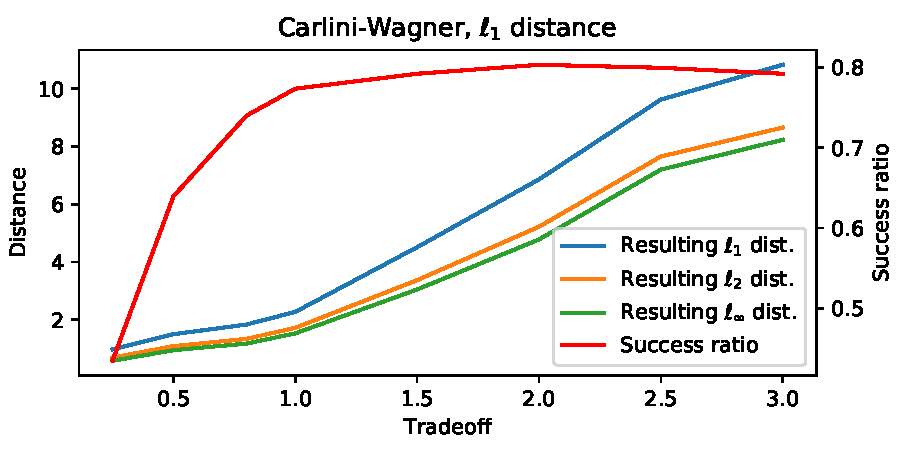
\includegraphics[width=0.45\textwidth]{adv_plots/cwl1.pdf}
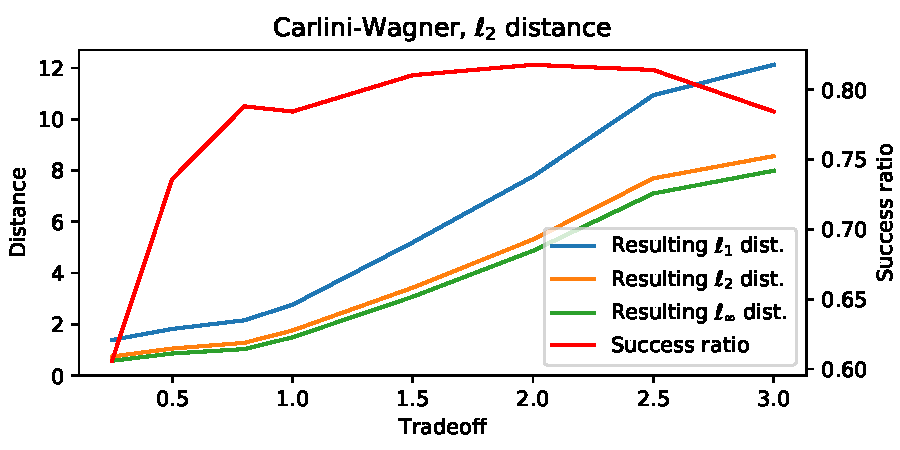
\includegraphics[width=0.45\textwidth]{adv_plots/cwl2.pdf}
\caption{Performance of the Carlini-Wagner method with different $\epsilon$ values for $\ell_1$ and $\ell_2$ distances.}
\label{fig:adv_cw}
\end{figure*}
\autoref{fig:adv_cw} depicts the ratio of attack flows which were successfully misclassified as normal traffic with respect to the final packet along with the resulting distance from the original sample. Evidently, the larger the $\epsilon$ parameter, the better the attack works, but also the distances become larger.

Hence, with acceptable distance values we were able to generate adversarial samples for about 80\% of attack samples.

The figure suggests that a tradeoff value between 0.5 and 1 would be ideal to find adversarial samples with a low enough distance from real samples. This conclusion might be misleading, however, as the distance cannot become larger anymore as soon as an adversarial sample has been found, when performing optimization as depicted by the objective function \eqref{eq:carliniWagner}. Hence, the depicted increase of average distances presumably is due to samples for which no adversarial sample was found for lower $\epsilon$ values.


\begin{table*}
\caption{Attack success ratios per attack family. Depicted are flow detection accuracies for adversarial flows (left numbers) and flow detection accuracies for unmodified flows (right numbers).}
\label{tab:adv_per_family}
\begin{tabular}{lllllllll}
\toprule
Attack type & FGSM & Carlini-Wagner, $\ell_1$ & Carlini-Wagner, $\ell_2$ & $\ell_\infty$-bounded PGD \\
\midrule
Botnet:ARES	&	0.0000 / 0.0000	&	0.0000 / 0.0000	&	0.0000 / 0.0000	&	0.0000 / 0.0000	\\
Brute Force:FTP-Patator	&	0.2800 / 0.5800	&	0.1600 / 0.5800	&	0.1600 / 0.5800	&	0.2800 / 0.5800	\\
Brute Force:SSH-Patator	&	0.8300 / 1.0000	&	0.0000 / 1.0000	&	0.0000 / 1.0000	&	0.8900 / 1.0000	\\
DDoS:LOIT	&	0.8300 / 0.8600	&	0.6400 / 0.8600	&	0.5600 / 0.8600	&	0.8200 / 0.8600	\\
DoS / DDoS:DoS GoldenEye	&	0.8900 / 1.0000	&	0.5000 / 1.0000	&	0.4200 / 1.0000	&	0.9200 / 1.0000	\\
DoS / DDoS:DoS Hulk	&	0.6700 / 1.0000	&	0.5400 / 1.0000	&	0.4700 / 1.0000	&	1.0000 / 1.0000	\\
DoS / DDoS:DoS Slowhttptest	&	0.8700 / 1.0000	&	0.4100 / 1.0000	&	0.1900 / 1.0000	&	0.7400 / 1.0000	\\
DoS / DDoS:DoS slowloris	&	0.4400 / 0.9700	&	0.3100 / 0.9700	&	0.1300 / 0.9700	&	0.9200 / 0.9700	\\
DoS / DDoS:Heartbleed	&	0.0000 / 0.0000	&	0.0000 / 0.0000	&	0.0000 / 0.0000	&	0.0000 / 0.0000	\\
Infiltration:Dropbox download 	&	0.6100 / 0.9600	&	0.4300 / 0.9600	&	0.3800 / 0.9600	&	0.7400 / 0.9600	\\
PortScan:PortScan - Firewall off	&	0.6800 / 0.9100	&	0.3500 / 0.9100	&	0.3500 / 0.9100	&	0.7200 / 0.9100	\\
PortScan:PortScan - Firewall on	&	0.7400 / 0.8700	&	0.6100 / 0.8700	&	0.5300 / 0.8700	&	0.7300 / 0.8700	\\
Web Attack:Sql Injection	&	0.0000 / 0.6923	&	0.0000 / 0.6923	&	0.0000 / 0.6923	&	0.0000 / 0.6923	\\
Web Attack:XSS	&	0.6700 / 0.9500	&	0.7200 / 0.9500	&	0.6200 / 0.9500	&	0.6700 / 0.9500	\\
\bottomrule

\end{tabular}
\end{table*}

It is interesting to note that for very large values of $\epsilon$ the success ratio starts to decrease again.This phenomenon might be due to numerical effects and might be preventable by a smaller learning rate.


\autoref{fig:fgsm} depicts the performance for FGSM and $\ell_\infty$-bounded PGD. As expected, while FGSM is the fastest of all algorithms, it delivers the worst performance.

Of the investigated algorithms, thus the Carlini-Wagner method with $\ell_2$ distance delivered the best performance.

\autoref{tab:adv_per_family} depicts how successful the attack is for individual attack families. For this table we used a $\ell_\infty$ bound of 0.3 for FGSM and $\ell_\infty$-bounded PGD and a tradeoff of 0.5 for Carlini-Wagner. The table shows significant for detecting different attack families in the first place. However, also for generating adversarial flows some attack families are more susceptible than others.

\begin{figure*}
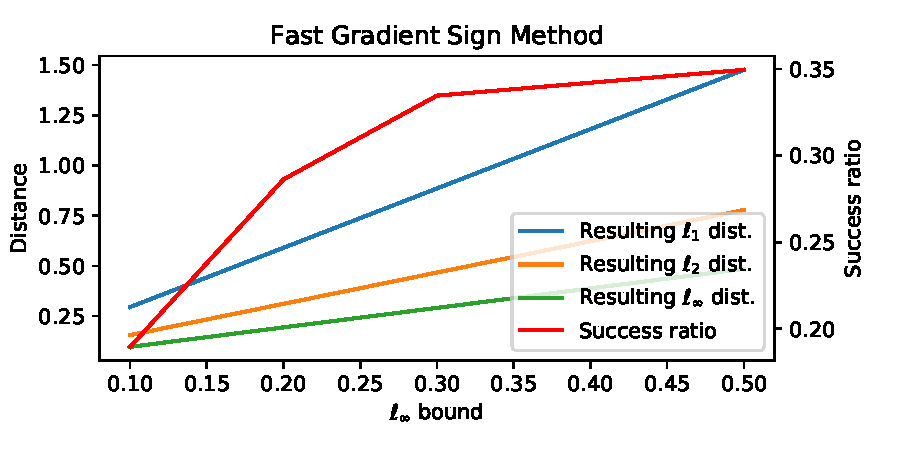
\includegraphics[width=0.45\textwidth]{adv_plots/fgsm.pdf}
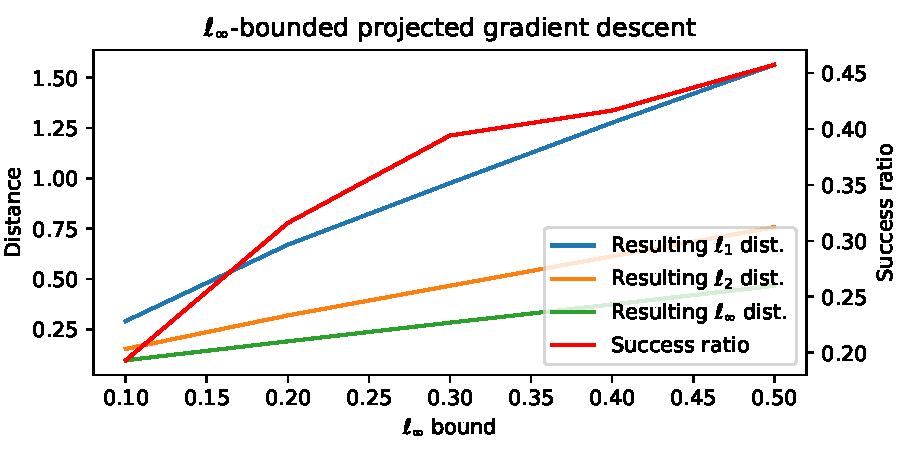
\includegraphics[width=0.45\textwidth]{adv_plots/l_inf_pgd.pdf}
\caption{Performance of FSGM and $\ell_\infty$-bounded PGD for different bounds.}
\label{fig:fgsm}
\end{figure*}

Finally, we investigated what adversarial flows look like and which features are manipulated to circumvent detection by the neural network.

To this end, we generated adversarial flows with the Carlini-Wagner method with $\ell_2$ distance and a tradeoff of 0.5. \autoref{adv_plots} depicts how the method manipulates flows for some exemplary attack categories. Depicted is the mean of both unmodified flows and adversarial flows  of samples of individual attack families considering both interarrival time and packet length.

The plots show that primarily features at the beginning of flows are modified. It is remarkable that it seems most promising to modifiy single packets while leaving most of the flow unchanged. In other cases, however, like depicted for the infiltration attack at the bottom, adversarial flows assume a complex pattern to circumvent detection.

\begin{figure*}[p]
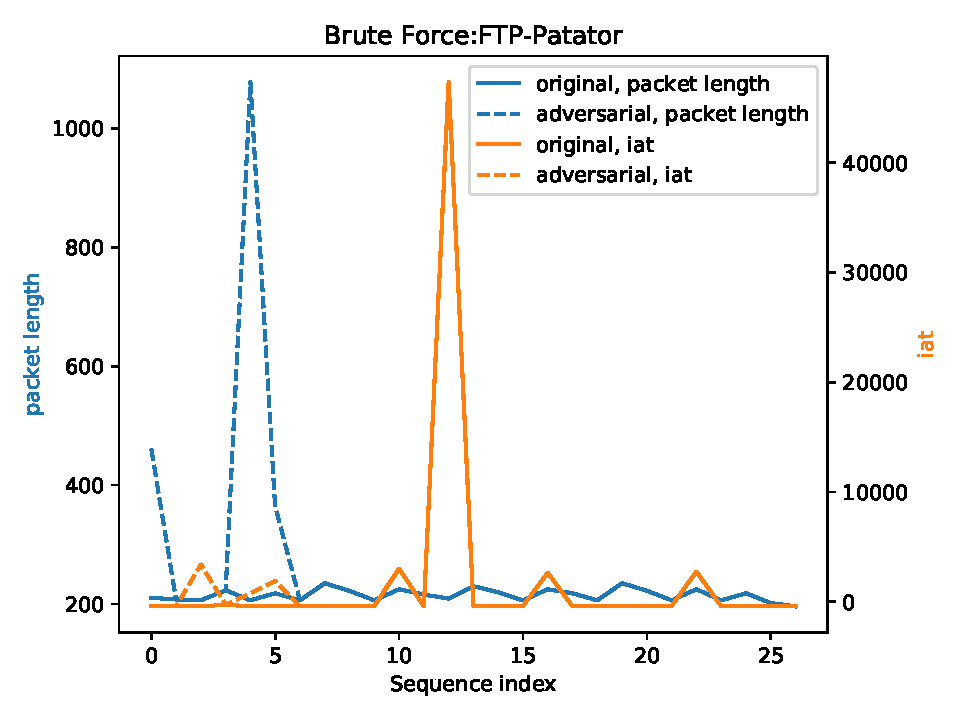
\includegraphics[width=0.48\textwidth]{../plots/plot_adv/1.pdf}
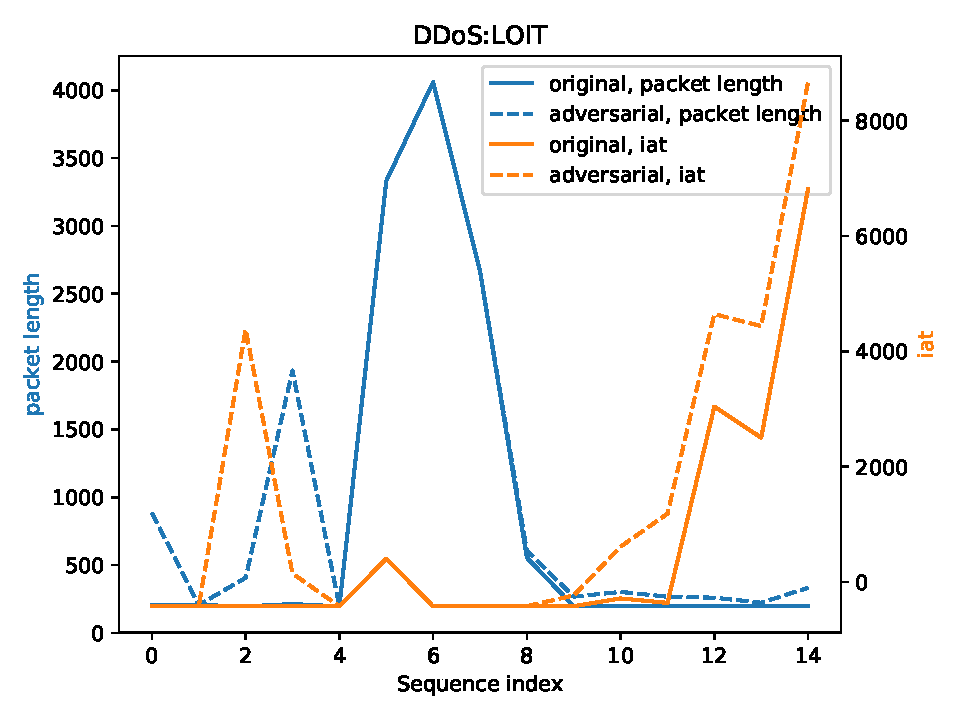
\includegraphics[width=0.48\textwidth]{../plots/plot_adv/2.pdf}
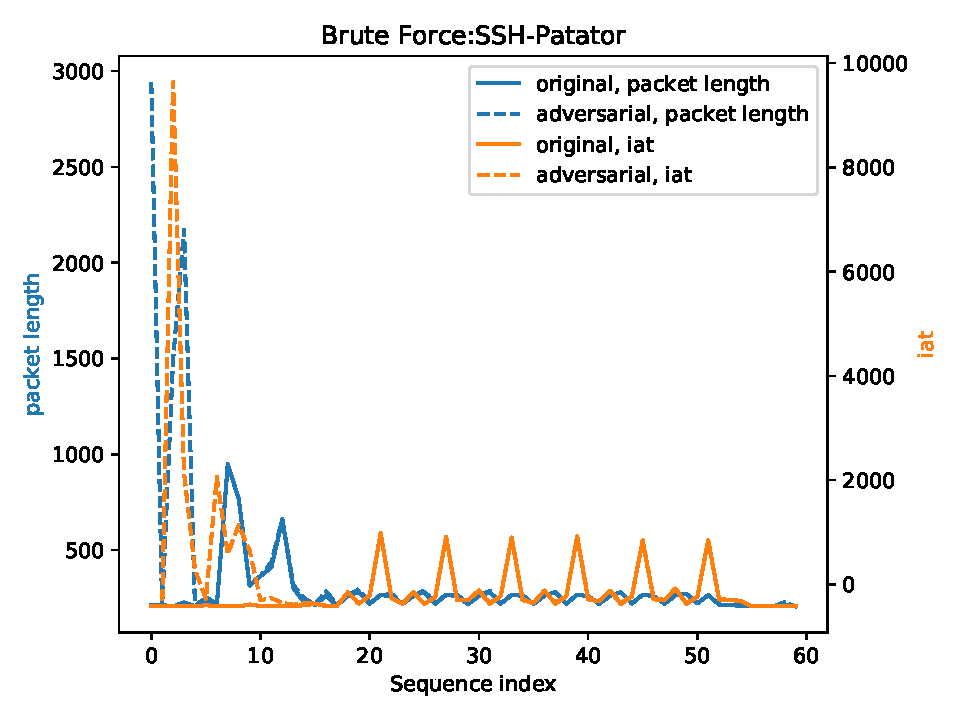
\includegraphics[width=0.48\textwidth]{../plots/plot_adv/3.pdf}
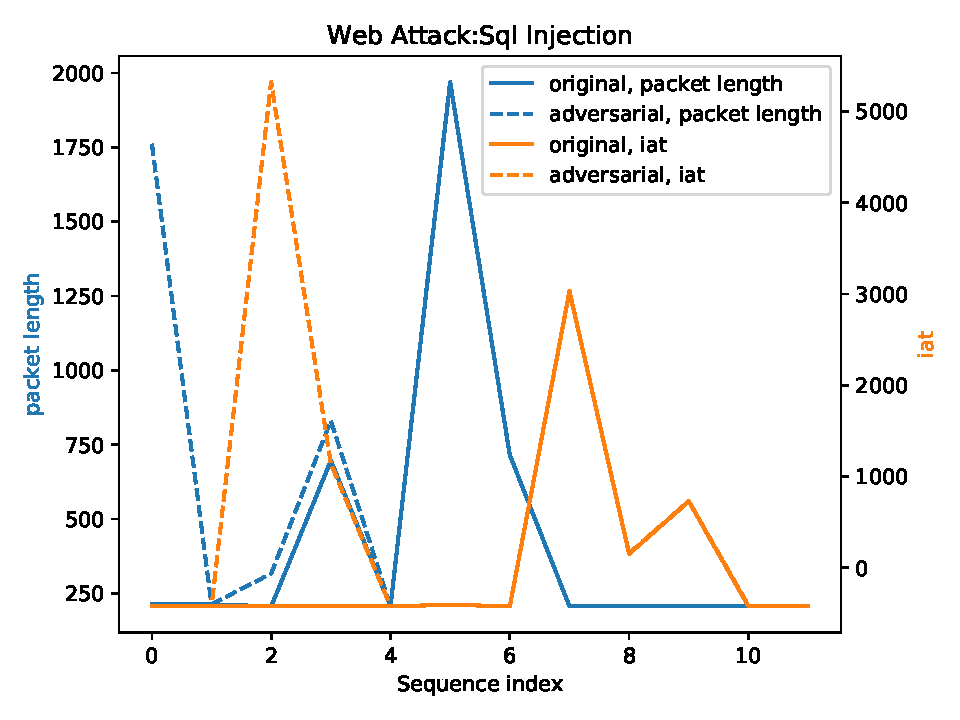
\includegraphics[width=0.48\textwidth]{../plots/plot_adv/4.pdf}
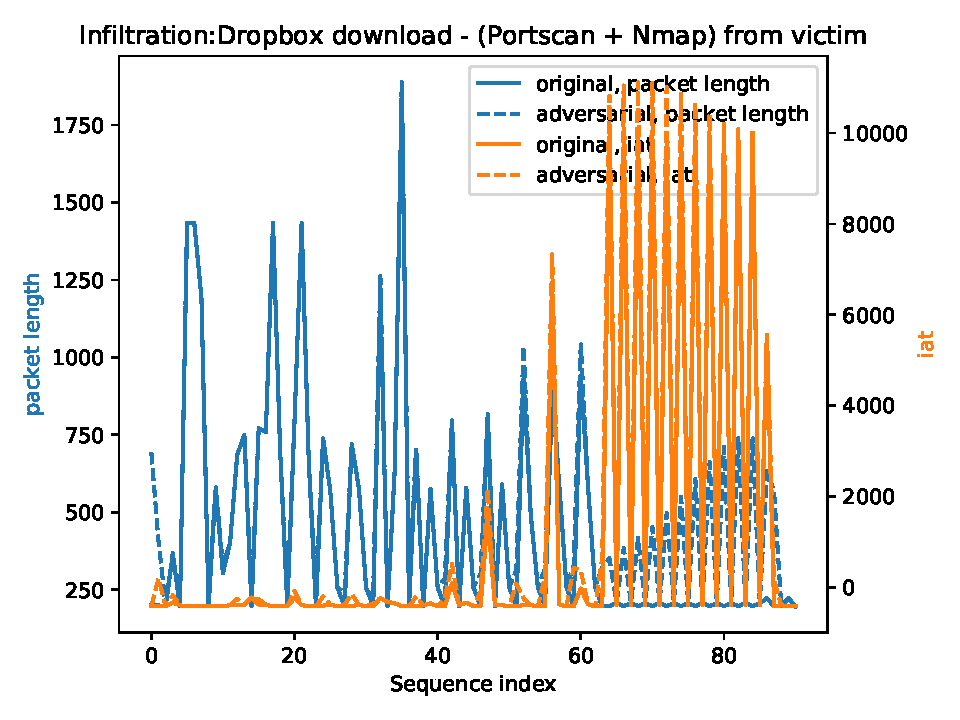
\includegraphics[width=0.48\textwidth]{../plots/plot_adv/5.pdf}
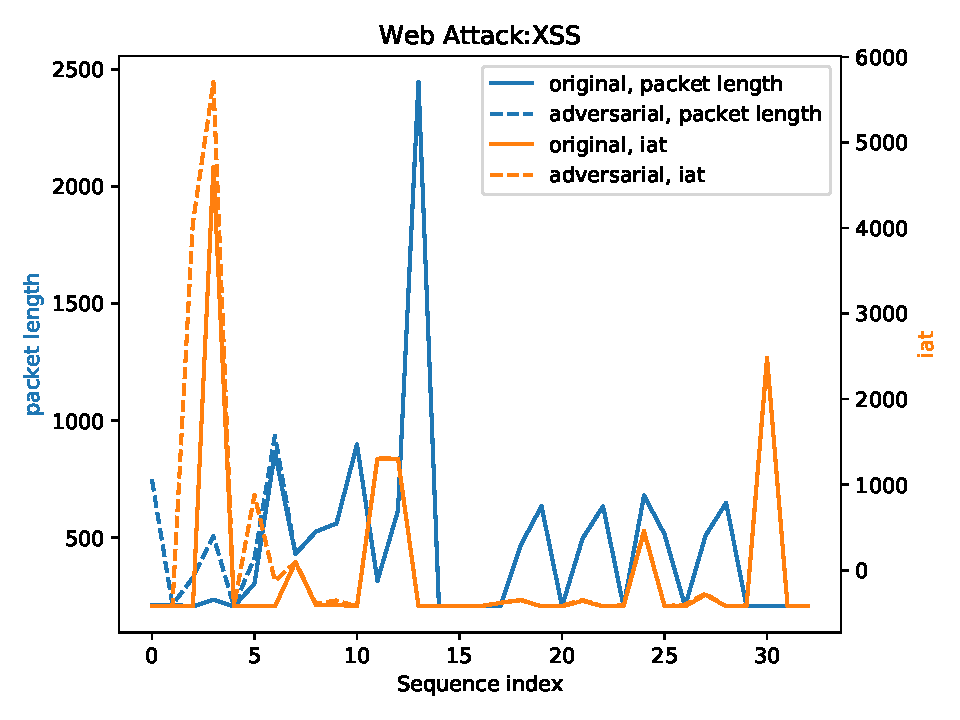
\includegraphics[width=0.48\textwidth]{../plots/plot_adv/6.pdf}
\caption{Successful manipulations performed by the Carlini-Wagner method.}
\label{adv_plots}
\end{figure*}


\subsection{Defences}

The most obvious defence, which is only possible because of the nature of the dataset, is to simply leave out features which the attacker can manipulate. For this, we try two different approaches:
\begin{itemize}
\item Leaving out all features that are manipulable: packet size and interarrival time
\item Leaving out manipulable features when the attacker can manipulate them: only in the direction from the attacker to the victim (This, however does not prevent adversarial samples for botnets, for which both sides are malicious)
\end{itemize}

Both approaches lead to complete resistance to adversarial samples (as we left out all manipulable features), except for botnets, which can still operate when only leaving out manipulable features in one direction. The results in \autoref{tab:performance_results_no_manipulable} show that -- surprisingly -- there is only a small difference in classification performance when only computing the accuracy for the last packet of each flow (flow accuracy). However, when looking at the packet accuracy, which considers all packets of all flows, there is a significant difference. Thus, apparently the interarrival time and packet size are especially important for determining whether a flow is malicious in the first packets of a flow.

In addition to omitting manipulable features we tried to make our network more robust against adversarial samples by augmenting the training set by adversarial flows generated using the Carlini-Wagner method, labelled as additional attacks. However, against our expectations, this approach did not lead to satisfactory results in the sense that the network would learn to classify adversarial samples as attacks. In fact, classification accuracy stayed about constant during the training of the network.

A possible explanation for this observation might be that the adversarial samples assumed too much the shape of normal flows, so that the network could not reliable tell them apart.

\begin{table*}
\caption{Comparing performance with all features, only safe features (interarrival time and packet size removed) and safe features in one direction (interarrival time and packet size removed for packets coming from source). \textit{packets} means that we consider the neural network output of all packets of the flow while \textit{flows} means that we only consider the last packet. At the last packet the classifier is usually already a lot more confident than at the first packets of a flow and thus metrics are always better in this case.}  \label{tab:performance_results_no_manipulable}
\newcommand{\cmidrulespace}{6pt}
\begin{tabular}{l l l l l l l} \toprule
& \multicolumn{2}{l}{all} & \multicolumn{2}{l}{safe features} & \multicolumn{2}{l}{safe features one direction} \\
\cmidrule(r){2-3} \cmidrule(lr){4-5} \cmidrule(l){6-7}
& packets & flows & packets & flows & packets & flows \\
\midrule
Accuracy & 0.9857054 & 0.99472587 & 0.96678023 & 0.99337596 & 0.98056073 & 0.99353386 \\
Precision & 0.94963342 & 0.9894422 & 0.87175275 & 0.98798596 & 0.91359787 & 0.98994595 \\
Recall & 0.96735895 & 0.98972051 & 0.94374958 & 0.98581328 & 0.97836672 & 0.9844478 \\
F1 & 0.95841423 & 0.98958134 & 0.90632359 & 0.98689842 & 0.94487366 & 0.98718922 \\
Youden & 0.95682951 & 0.98614231 & 0.91525628 & 0.98175163 & 0.95937772 & 0.9810602 \\
\bottomrule
\end{tabular}
\end{table*}

\section{Conclusions}

We have implemented a recurrent classifier based on LSTM to detect network attacks. While attack detection performance is not better than that of non-recurrent approaches, we can already detect attacks before they are over. Furthermore, the recurrent approach allows us to inspect the influence of single packets on the detection performance and shows which packets are \textit{characteristic} for attacks.

We show that adversarial samples are possible even though the data we use are very different from those that are usually used when finding adversarial samples.

\bibliographystyle{ACM-Reference-Format}
\bibliography{bibliography}


\end{document}
\endinput
%%
%% End of file `sample-sigconf.tex'.
